\documentclass[tikz,border=10pt]{standalone}
\usepackage{amsmath}

\begin{document}
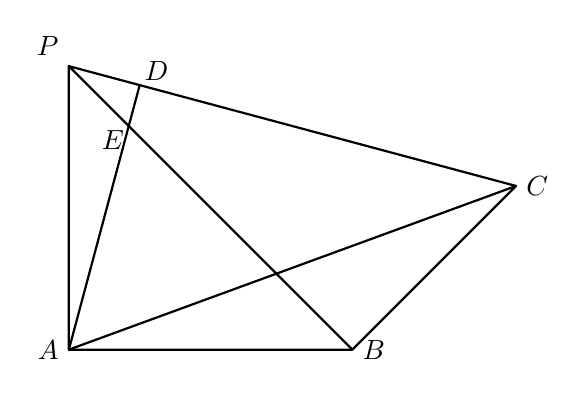
\begin{tikzpicture}[scale=1.2, thick, >=stealth, line join=round, line cap=round]

    % --- 1. 定义平面展开后的精确坐标 ---
    \coordinate (A) at (0,0);
    \coordinate (B) at (3,0);
    \coordinate (P) at (0,3);
    % 经过严格角度计算展开后的 C 点位置
    \coordinate (C) at (4.732, 1.732);

    % --- 2. 定义垂直最值点坐标 ---
    \coordinate (D) at (0.75, 2.80);
    \coordinate (E) at (0.634, 2.366);

    % --- 3. 绘制展开面的实线轮廓 ---
    \draw (A) -- (B) -- (C) -- (P) -- cycle;
    
    % --- 4. 绘制内部辅助与最值连线 ---
    \draw (P) -- (B);
    \draw (A) -- (C);
    \draw (A) -- (D); % 最短距离的垂线

    % --- 5. 节点字母标定 ---
    \node[left] at (A) {$A$};
    \node[right] at (B) {$B$};
    \node[above left] at (P) {$P$};
    \node[right] at (C) {$C$};
    \node[above right, xshift=-2pt, yshift=-2pt] at (D) {$D$};
    \node[below left, xshift=2pt, yshift=2pt] at (E) {$E$};

\end{tikzpicture}
\end{document}